\documentclass{article}
\usepackage[utf8]{inputenc}
\usepackage[T1]{fontenc}
\usepackage[a4paper, margin=0.5in]{geometry}
\usepackage{amssymb}
\usepackage{amsmath}
\usepackage{amsfonts}
\usepackage{xcolor}
\usepackage{multirow}
\usepackage{graphicx}
\usepackage{fancyhdr}
\pagestyle{plain}

\newcommand*{\TIMEOUT}{--}
\newcommand*{\ERROR}{unk}
\newcommand*{\unk}{unk}
\newcommand*{\ERR}{\ERROR}

\begin{document}

\begin{table}
\centering\scriptsize
\caption{Overall results.}
\begin{tabular}{|p{5em}||c|c|c|c||c|c|}\hline
Synthesis & Rab & Tem & RPG & T2R & S$_{\textit{acc}}$ & S \\\hline
    solved & 0 & 0 & 0 & 0 & \textbf{2} & 0\\
    best & 0 & 0 & 0 & 0 & \textbf{2} & 0\\
    unique & 0 & 0 & 0 & 0 & \textbf{2} & 0\\\hline
\end{tabular}\\
\begin{tabular}{|p{6.2em}||c|c|c||c|c|}\hline
Realisability & RPG & RSt & T2R & S$_{\textit{acc}}$ & S \\\hline
    solved & 0 & 0 & 0 & \textbf{2} & 0\\
    best & 0 & 0 & 0 & \textbf{2} & 0\\
    unique & 0 & 0 & 0 & \textbf{2} & 0\\\hline
\end{tabular}

\end{table}

\begin{table}
    \centering\scriptsize
    \caption{LTL benchmarks.}\label{tab:ltl}
    \begin{tabular}{|c|c||c|c|}
\hline
\multirow{2}{*}{Name} & \multirow{2}{*}{U} & \multicolumn{2}{c|}{Time (s)}\\\cline{3-4}
& & S$_{\textit{acc}}$ & S\\\hline\hline
\textsf{arbiter} & {} &  & \\\hline
\textsf{arbiter-failure} & {} &  & \\\hline
\textsf{elevator} & {} &  & \\\hline
\textsf{infinite-race} & {} &  & \\\hline
\textsf{infinite-race-u} & {$\bullet$} &  & \\\hline
\textsf{infinite-race-unequal-1} & {} &  & \\\hline
\textsf{infinite-race-unequal-2} & {} &  & \\\hline
\textsf{reversible-lane-r} & {} &  & \\\hline
\textsf{reversible-lane-u} & {$\bullet$} &  & \\\hline
\textsf{rep-reach-obst-1d} & {} &  & \\\hline
\textsf{rep-reach-obst-2d} & {} &  & \\\hline
\textsf{rep-reach-obst-6d} & {} &  & \\\hline
\textsf{robot-collect-v4} & {} &  & \\\hline
\textsf{taxi-service} & {} &  & \\\hline
\textsf{taxi-service-u} & {$\bullet$} &  & \\\hline

\end{tabular}
\end{table}

\begin{table}
\centering\scriptsize
\caption{%
    Experimental evaluation on
    \textbf{RPG}solve,
    \textbf{R}PG-\textbf{St}eLA,
    \textbf{T}slmt\textbf{2R}pg,
    \textbf{Rab}oniel,
    \textbf{Tem}os,
    and our \textbf{S}ynthesis tool
    (with and without \emph{acc}eleration).
    \textbf{U}~marks unrealisable instances.
    \TIMEOUT\ denotes timeout,
    \ERROR\ an error or inconclusive result,
    \textsf{x} an incorrect verdict.
    The best synthesis times are set in bold. 
    }\label{tab:results}
    
\begin{tabular}{|c|lr|c||c|c|c||c|c|c|c||c|c|}\hline
\multirow{2}{*}{G.}
& \multirow{2}{*}{Name, source} &
& \multirow{2}{*}{U}
& \multicolumn{3}{c||}{Realisability (s)}
& \multicolumn{6}{c|}{Synthesis (s)}\\\cline{5-13}
& & & & RPG & T2R & RSt & RPG & T2R & Rab & Tem & S$_{\textit{acc}}$ & S\\\hline\hline
\multirow{11}{*}{\rotatebox[origin=c]{90}{Safety}}
&  \textsf{box} & \cite{10.1145/3632899} &  &  &  &  &  &  &  &  &  &  \\
&  \textsf{box-limited} & \cite{10.1145/3632899} &  &  &  &  &  &  &  &  & \textbf{3.26} &  \\
&  \textsf{diagonal} & \cite{10.1145/3632899} &  &  &  &  &  &  &  &  &  &  \\
&  \textsf{evasion} & \cite{10.1145/3632899} &  &  &  &  &  &  &  &  &  &  \\
&  \textsf{follow} & \cite{10.1145/3632899} &  &  &  &  &  &  &  &  &  &  \\
&  \textsf{solitary} & \cite{10.1145/3632899} &  &  &  &  &  &  &  &  &  &  \\
&  \textsf{square} & \cite{10.1145/3632899} &  &  &  &  &  &  &  &  &  &  \\
&  \textsf{g-real} & \cite{DBLP:journals/pacmpl/HeimD25} &  &  &  &  &  &  &  &  &  &  \\
&  \textsf{g-unreal-1} & \cite{DBLP:journals/pacmpl/HeimD25} & $\bullet$ &  &  &  &  &  &  &  &  &  \\
&  \textsf{g-unreal-2} & \cite{DBLP:journals/pacmpl/HeimD25} & $\bullet$ &  &  &  &  &  &  &  &  &  \\
&  \textsf{g-unreal-3} & \cite{DBLP:journals/pacmpl/HeimD25} & $\bullet$ &  &  &  &  &  &  &  &  &  \\
\hline\hline
\multirow{25}{*}{\rotatebox[origin=c]{90}{Reachability}}
&  \textsf{heim-double-x} & \cite{10.1145/3632899} &  &  &  &  &  &  &  &  &  &  \\
&  \textsf{robot-cat-real-1d} & \cite{10.1145/3632899} &  &  &  &  &  &  &  &  &  &  \\
&  \textsf{robot-cat-unreal-1d} & \cite{10.1145/3632899} & $\bullet$ &  &  &  &  &  &  &  &  &  \\
&  \textsf{robot-cat-real-2d} & \cite{10.1145/3632899} &  &  &  &  &  &  &  &  &  &  \\
&  \textsf{robot-cat-unreal-2d} & \cite{10.1145/3632899} & $\bullet$ &  &  &  &  &  &  &  &  &  \\
&  \textsf{robot-grid-reach-1d} & \cite{10.1145/3632899} &  &  &  &  &  &  &  &  &  &  \\
&  \textsf{robot-grid-reach-2d} & \cite{10.1145/3632899} &  &  &  &  &  &  &  &  &  &  \\
&  \textsf{sort4} & \cite{DBLP:conf/isola/MaderbacherWB24} &  &  &  &  &  &  &  &  &  &  \\
&  \textsf{sort5} & \cite{DBLP:conf/isola/MaderbacherWB24} &  &  &  &  &  &  &  &  &  &  \\
&  \textsf{F-G-contradiction-1} & \cite{DBLP:journals/pacmpl/HeimD25} & $\bullet$ &  &  &  &  &  &  &  &  &  \\
&  \textsf{F-G-contradiction-2} & \cite{DBLP:journals/pacmpl/HeimD25} & $\bullet$ &  &  &  &  &  &  &  &  &  \\
&  \textsf{f-real} & \cite{DBLP:journals/pacmpl/HeimD25} &  &  &  &  &  &  &  &  &  &  \\
&  \textsf{f-unreal} & \cite{DBLP:journals/pacmpl/HeimD25} & $\bullet$ &  &  &  &  &  &  &  &  &  \\
&  \textsf{ordered-visits} & \cite{DBLP:journals/pacmpl/HeimD25} &  &  &  &  &  &  &  &  &  &  \\
&  \textsf{ordered-visits-choice} & \cite{DBLP:journals/pacmpl/HeimD25} &  &  &  &  &  &  &  &  &  &  \\
&  \textsf{precise-reachability} & \cite{DBLP:journals/pacmpl/HeimD25} &  &  &  &  &  &  &  &  &  &  \\
&  \textsf{robot-to-target} & \cite{DBLP:journals/pacmpl/HeimD25} &  &  &  &  &  &  &  &  &  &  \\
&  \textsf{robot-to-target-unreal} & \cite{DBLP:journals/pacmpl/HeimD25} & $\bullet$ &  &  &  &  &  &  &  &  &  \\
&  \textsf{robot-to-target-charging} & \cite{DBLP:journals/pacmpl/HeimD25} &  &  &  &  &  &  &  &  &  &  \\
&  \textsf{robot-to-target-charging-unreal} & \cite{DBLP:journals/pacmpl/HeimD25} & $\bullet$ &  &  &  &  &  &  &  &  &  \\
&  \textsf{thermostat-F} & \cite{DBLP:journals/pacmpl/HeimD25} &  &  &  &  &  &  &  &  &  &  \\
&  \textsf{thermostat-F-unreal} & \cite{DBLP:journals/pacmpl/HeimD25} & $\bullet$ &  &  &  &  &  &  &  &  &  \\
&  \textsf{unordered-visits-charging} & \cite{DBLP:journals/pacmpl/HeimD25} &  &  &  &  &  &  &  &  &  &  \\
&  \textsf{unordered-visits} & \cite{DBLP:journals/pacmpl/HeimD25} &  &  &  &  &  &  &  &  &  &  \\
&  \textsf{robot-tasks} &  &  &  &  &  &  &  &  &  & \textbf{2.77} &  \\
\hline\hline
\multirow{45}{*}{\rotatebox[origin=c]{90}{Deterministic B\"uchi}}
&  \textsf{heim-buechi} & \cite{10.1145/3632899} &  &  &  &  &  &  &  &  &  &  \\
&  \textsf{heim-fig7} & \cite{10.1145/3632899} & $\bullet$ &  &  &  &  &  &  &  &  &  \\
&  \textsf{robot-commute-1d} & \cite{10.1145/3632899} &  &  &  &  &  &  &  &  &  &  \\
&  \textsf{robot-commute-2d} & \cite{10.1145/3632899} &  &  &  &  &  &  &  &  &  &  \\
&  \textsf{robot-resource-1d} & \cite{10.1145/3632899} & $\bullet$ &  &  &  &  &  &  &  &  &  \\
&  \textsf{robot-resource-2d} & \cite{10.1145/3632899} & $\bullet$ &  &  &  &  &  &  &  &  &  \\
&  \textsf{chain-4} & \cite{DBLP:conf/cav/SchmuckHDN24} &  &  &  &  &  &  &  &  &  &  \\
&  \textsf{chain-5} & \cite{DBLP:conf/cav/SchmuckHDN24} &  &  &  &  &  &  &  &  &  &  \\
&  \textsf{chain-6} & \cite{DBLP:conf/cav/SchmuckHDN24} &  &  &  &  &  &  &  &  &  &  \\
&  \textsf{chain-7} & \cite{DBLP:conf/cav/SchmuckHDN24} &  &  &  &  &  &  &  &  &  &  \\
&  \textsf{chain-simple-5} & \cite{DBLP:conf/cav/SchmuckHDN24} &  &  &  &  &  &  &  &  &  &  \\
&  \textsf{chain-simple-10} & \cite{DBLP:conf/cav/SchmuckHDN24} &  &  &  &  &  &  &  &  &  &  \\
&  \textsf{chain-simple-20} & \cite{DBLP:conf/cav/SchmuckHDN24} &  &  &  &  &  &  &  &  &  &  \\
&  \textsf{chain-simple-30} & \cite{DBLP:conf/cav/SchmuckHDN24} &  &  &  &  &  &  &  &  &  &  \\
&  \textsf{chain-simple-40} & \cite{DBLP:conf/cav/SchmuckHDN24} &  &  &  &  &  &  &  &  &  &  \\
&  \textsf{chain-simple-50} & \cite{DBLP:conf/cav/SchmuckHDN24} &  &  &  &  &  &  &  &  &  &  \\
&  \textsf{chain-simple-60} & \cite{DBLP:conf/cav/SchmuckHDN24} &  &  &  &  &  &  &  &  &  &  \\
&  \textsf{chain-simple-70} & \cite{DBLP:conf/cav/SchmuckHDN24} &  &  &  &  &  &  &  &  &  &  \\
&  \textsf{items-processing} & \cite{DBLP:conf/cav/SchmuckHDN24} &  &  &  &  &  &  &  &  &  &  \\
&  \textsf{robot-analyze} & \cite{DBLP:conf/cav/SchmuckHDN24} &  &  &  &  &  &  &  &  &  &  \\
&  \textsf{robot-collect-v1} & \cite{DBLP:conf/cav/SchmuckHDN24} &  &  &  &  &  &  &  &  &  &  \\
&  \textsf{robot-collect-v2} & \cite{DBLP:conf/cav/SchmuckHDN24} &  &  &  &  &  &  &  &  &  &  \\
&  \textsf{robot-collect-v3} & \cite{DBLP:conf/cav/SchmuckHDN24} &  &  &  &  &  &  &  &  &  &  \\
&  \textsf{robot-deliver-v1} & \cite{DBLP:conf/cav/SchmuckHDN24} &  &  &  &  &  &  &  &  &  &  \\
&  \textsf{robot-deliver-v2} & \cite{DBLP:conf/cav/SchmuckHDN24} &  &  &  &  &  &  &  &  &  &  \\
&  \textsf{robot-deliver-v3} & \cite{DBLP:conf/cav/SchmuckHDN24} &  &  &  &  &  &  &  &  &  &  \\
&  \textsf{robot-deliver-v4} & \cite{DBLP:conf/cav/SchmuckHDN24} &  &  &  &  &  &  &  &  &  &  \\
&  \textsf{robot-deliver-v5} & \cite{DBLP:conf/cav/SchmuckHDN24} &  &  &  &  &  &  &  &  &  &  \\
&  \textsf{robot-repair} & \cite{DBLP:conf/cav/SchmuckHDN24} &  &  &  &  &  &  &  &  &  &  \\
&  \textsf{robot-running} & \cite{DBLP:conf/cav/SchmuckHDN24} &  &  &  &  &  &  &  &  &  &  \\
&  \textsf{scheduler} & \cite{DBLP:conf/cav/SchmuckHDN24} &  &  &  &  &  &  &  &  &  &  \\
&  \textsf{buffer-storage} & \cite{DBLP:journals/pacmpl/HeimD25} &  &  &  &  &  &  &  &  &  &  \\
&  \textsf{gf-real} & \cite{DBLP:journals/pacmpl/HeimD25} &  &  &  &  &  &  &  &  &  &  \\
&  \textsf{gf-unreal} & \cite{DBLP:journals/pacmpl/HeimD25} & $\bullet$ &  &  &  &  &  &  &  &  &  \\
&  \textsf{GF-G-contradiction} & \cite{DBLP:journals/pacmpl/HeimD25} & $\bullet$ &  &  &  &  &  &  &  &  &  \\
&  \textsf{helipad} & \cite{DBLP:journals/pacmpl/HeimD25} &  &  &  &  &  &  &  &  &  &  \\
&  \textsf{helipad-contradict} & \cite{DBLP:journals/pacmpl/HeimD25} & $\bullet$ &  &  &  &  &  &  &  &  &  \\
&  \textsf{package-delivery} & \cite{DBLP:journals/pacmpl/HeimD25} &  &  &  &  &  &  &  &  &  &  \\
&  \textsf{patrolling} & \cite{DBLP:journals/pacmpl/HeimD25} &  &  &  &  &  &  &  &  &  &  \\
&  \textsf{patrolling-alarm} & \cite{DBLP:journals/pacmpl/HeimD25} &  &  &  &  &  &  &  &  &  &  \\
&  \textsf{storage-GF-64} & \cite{DBLP:journals/pacmpl/HeimD25} &  &  &  &  &  &  &  &  &  &  \\
&  \textsf{tasks} & \cite{DBLP:journals/pacmpl/HeimD25} &  &  &  &  &  &  &  &  &  &  \\
&  \textsf{tasks-unreal} & \cite{DBLP:journals/pacmpl/HeimD25} & $\bullet$ &  &  &  &  &  &  &  &  &  \\
&  \textsf{thermostat-GF} & \cite{DBLP:journals/pacmpl/HeimD25} &  &  &  &  &  &  &  &  &  &  \\
&  \textsf{thermostat-GF-unreal} & \cite{DBLP:journals/pacmpl/HeimD25} & $\bullet$ &  &  &  &  &  &  &  &  &  \\
\hline
\end{tabular}

\end{table}

\begin{table}
    \caption{Experiment details for S{$_{acc}$} and S.}\label{tab:details}
    \centering\tiny
    \begin{tabular}[t]{|l||c||c|c|c|c|c|c||}
\hline
&& \multicolumn{2}{c|}{init}
& \multicolumn{2}{c|}{ref}
& \multicolumn{2}{c||}{add}\\\hline
\multicolumn{1}{|c||}{Name} & acc & s & t &sf. &sl. & sp & tp\\\hline\hline\multirow{2}{*}[0em]{box-limited}

& $\bullet$
& 2 & 2 & 0 & 0 & 0 & 0\\\cline{2-8}
& 
& -- & -- & -- & -- & -- & --\\\hline
\end{tabular}\begin{tabular}[t]{|l||c||c|c|c|c|c|c||}
\hline
&& \multicolumn{2}{c|}{init}
& \multicolumn{2}{c|}{ref}
& \multicolumn{2}{c||}{add}\\\hline
\multicolumn{1}{|c||}{Name} & acc & s & t &sf. &sl. & sp & tp\\\hline\hline\multirow{2}{*}[0em]{robot-tasks}

& $\bullet$
& 4 & 4 & 0 & 0 & 0 & 0\\\cline{2-8}
& 
& -- & -- & -- & -- & -- & --\\\hline
\end{tabular}
\end{table}
\clearpage

\centering
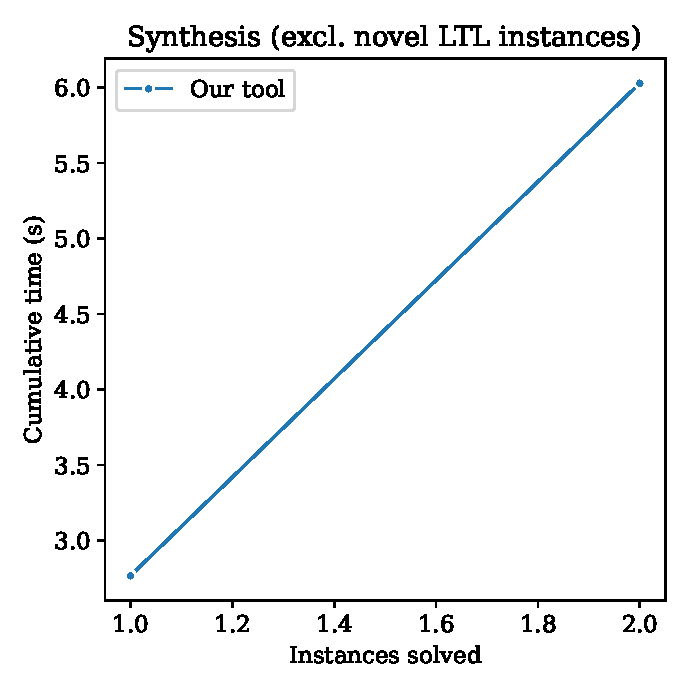
\includegraphics[width=0.4\textwidth]{cactus-syn.pdf}
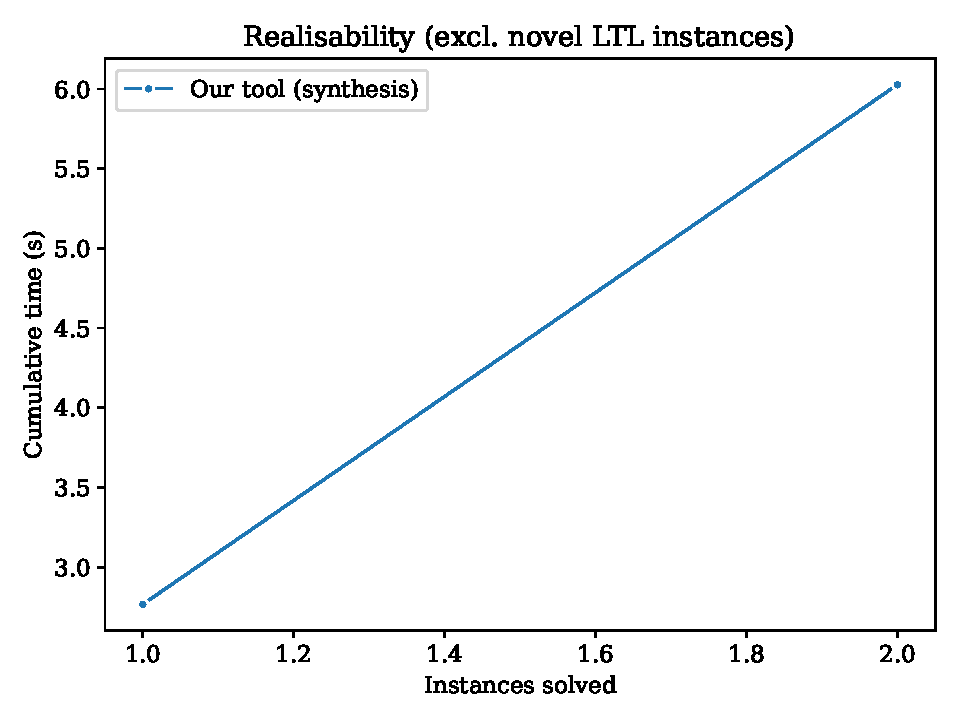
\includegraphics[width=0.4\textwidth]{cactus-real.pdf}

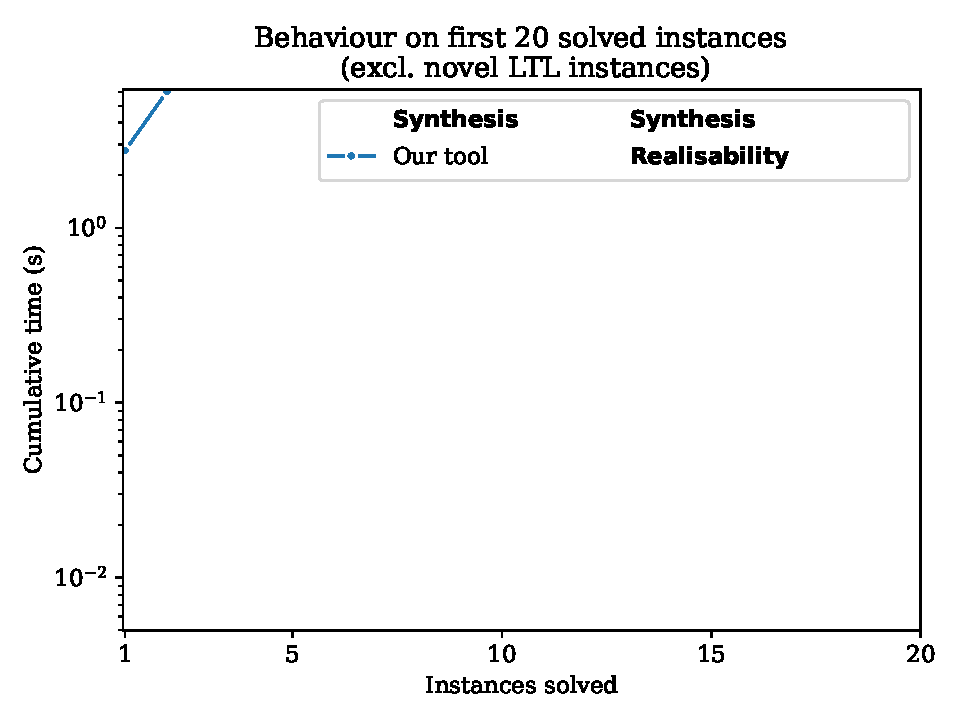
\includegraphics[width=0.7\textwidth]{cactus-easy.pdf}


\clearpage

\bibliographystyle{plain}
\bibliography{references}
\end{document}